\section{Considerações iniciais}
Neste capítulo os métodos de geração artificial para o rebalanceamento de classes
de imagens são descritos.

Foram realizados experimentos que são posteriormente descritos no Capítulo
\ref{cap:resultados} utilizando borramento, mistura ponderada, unsharp masking,
composição, combinação de thresholds, combinação com saliência, visual SMOTE e adição de ruído.

Dada a quantidade de imagens necessárias para rebalancear a base de imagens, foram geradas imagens utilizando
cada método, além de uma versão combinando todos eles (ou seja, algumas imagens de cada).

Pode-se verificar na imagem x que dado o conjunto de treinamento da classe (ou classes)
com menor número total de imagens, é realizado o rebalanceamento ao aplicar os
métodos descritos nesse capítulo e usar as imagens resultantes como treinamento.

%  \begin{figure}[hbpt]
%  \begin{center}
%    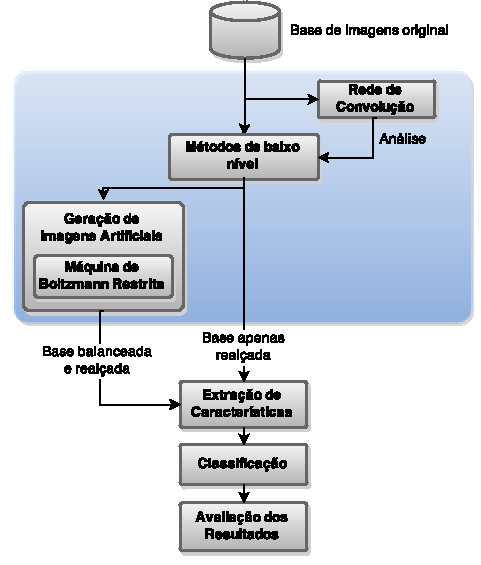
\includegraphics[width=1\linewidth]{\detokenize {figuras/geral.pdf}}
%  \end{center}
%   \caption[]{\textit{Fonte: Elaborado pela autora.}}
%  \label{fig:geral}
% \end{figure}

%%%%%%%%%%%%%%%%%%%%%%%%%%%%%%%%%%%%%%%%%%%%%%%%%%%%%%%%%%%%%%%%%%%%%%%%%%%%%%%%
\section{Borramento}
% \begin{espacosimples}

\begin{figure}
 \begin{center}
\begin{subfigure}{.45\textwidth}
  \centering
  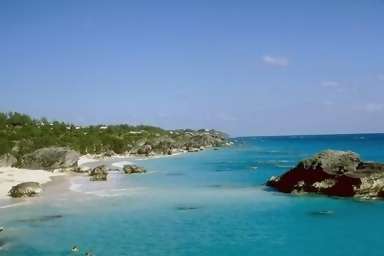
\includegraphics[width=\linewidth]{\detokenize{figuras/geracao/blur-a.png}}
  \caption{Original}
\end{subfigure}
\begin{subfigure}{.45\textwidth}
  \centering
  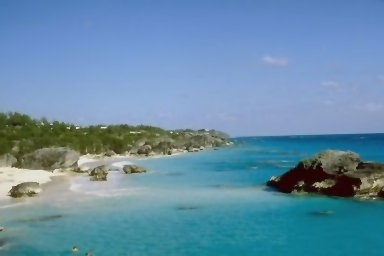
\includegraphics[width=\linewidth]{\detokenize{figuras/geracao/blur-b.png}}
  \caption{Imagem artificial}
\end{subfigure}
 \end{center}
 \caption[...]{\textit{Fonte:~Elaborado pela autora.}}
 \label{fig:gen:blur}
\end{figure}

Borramento, ou filtro de suavização, é uma operação de pré-processamento
comumente utilizada com o objetivo de reduzir ruído em uma imagem. Normalmente
esse tipo de filtro acarreta no borramento das bordas, como pode ser observado na
Figura \ref{fig:gren:blur}. Esse comportamento não é esperado quando devemos gerar novas imagens,
pois dessa forma há informação relevante que será removida.

Assim, a operação de borramento utilizada é a de filtro bilateral. Ela substitui
o valor do pixel $x$ com uma média dos pixeis de intensidade similar na imagem e dos pixeis
vizinhos \cite{Tomasi1998}.

\vspace{0.5cm}
\begin{algorithm}[H]
  \caption{Algoritmo de borramento com filtro bilateral}
  \label{alg:blur}
  \SetAlgoLined
  \Entrada{Imagem colorida $I$ em formato BGR}
  \Entrada{Diâmetro $d$ de pixinhança de pixels}
  \Entrada{Sigma do espaço de cor}
  \Entrada{Sigma do espaço de coordenadas}

  \Saida{Imagem gerada $G$}

  \meutodo{Algoritmo de filtro bilateral}
\end{algorithm}
\vspace{0.5cm}

\begin{description}
  \item[Parâmetros e suas variações] Conforme descrito no Algoritmo \ref{alg:blur},
os parâmetros para essa geração são: o diâmetro $d$ de pixinhança de pixels, o
$\sigma$ do espaço de cor e o $\sigma$ do espaço de coordenadas.

Esses parâmetros dependem das propriedades das imagens e dos resultados pretendidos.
Dessa forma, o tamanho do filtro é um valor escolhido arbitrariamente para cada
aplicação em específico \cite{Tomasi1998}. Como o nosso objetivo com a geração das
imagens não foi especializar no comportamento de uma classe de imagens específica,
um valor foi escolhido aleatoriamente e a partir dele os parâmetros de entrada
foram definidos.

\item[Limitações]

\item[Métodos relacionados]
São diversos os métodos de borramento descritos na literatura, como a filtragem
Gaussiana e a de mediana.

\item[Visualização]
É interessante notar na Figura x o comportamento da adição de rúido para rebalanceamento
em classes bem descritas pela propriedade da cor.

\meutodo{colocar aqui alguma figura do espaço}

\end{description}
%%%%%%%%%%%%%%%%%%%%%%%%%%%%%%%%%%%%%%%%%%%%%%%%%%%%%%%%%%%%%%%%%%%%%%%%%%%%%%%%
\section{Mistura ponderada}
\begin{figure}
 \begin{center}
\begin{subfigure}{.3\textwidth}
  \centering
  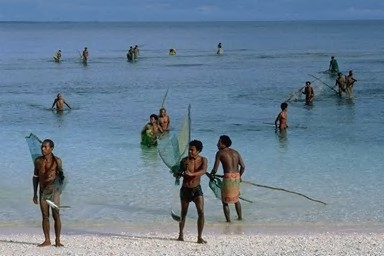
\includegraphics[width=\linewidth]{\detokenize{figuras/geracao/blend-a.png}}
  \caption{Original}
\end{subfigure}
\begin{subfigure}{.3\textwidth}
  \centering
  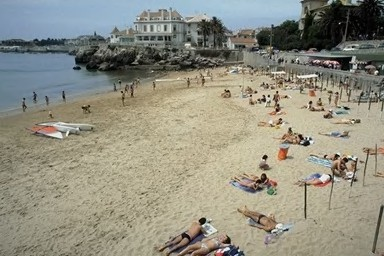
\includegraphics[width=\linewidth]{\detokenize{figuras/geracao/blend-b.png}}
  \caption{Original}
\end{subfigure}
\begin{subfigure}{.3\textwidth}
  \centering
  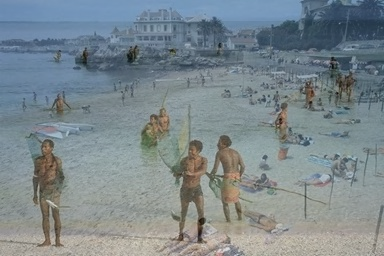
\includegraphics[width=\linewidth]{\detokenize{figuras/geracao/blend-c.png}}
  \caption{Imagem artificial}
\end{subfigure}
 \end{center}
 \caption[...]{\textit{Fonte:~Elaborado pela autora.}}
 \label{fig:gen:blend}
\end{figure}


Esse método calcula a soma ponderada de duas imagens e seu efeito pode ser visto na Figura \ref{fig:gen:blend}.


\vspace{0.5cm}
\begin{algorithm}[H]
  \caption{Algoritmo de mistura ponderada}
  \label{alg:blend}
  \SetAlgoLined
  \Entrada{Primeira imagem colorida $I$ em formato BGR}
  \Entrada{Segunda imagem colorida $I_2$ em formato BGR}

  \Saida{Imagem gerada $G$}

  {$\alpha \gets \text{número aletatório entre 10 e 80}$\;}
  {$\beta \gets 100 - \alpha$\;}

  \ParaCada{pixel $p$}{
    $\text{G}(p) \gets \beta.I(p) + \alpha.I_2$\;
  }
  \end{algorithm}
\vspace{0.5cm}

\begin{description}
\item[Parâmetros e suas variações]
Os parâmetros $\alpha$ e $\beta$ são escolhidos de forma aleatória. Um valor entre
10\% e 80\% é escolhido para $\alpha$ e o $\beta$ é o restante para completar 100\%.

\item[Limitações]
Não foi testado uma porcentagem fixa para verificar se existe algum ganho em utilizar
uma ponderação específica.

\item[Métodos relacionados]
É um método de combinação de imagens primitivo. Algoritmos similares são muito mais
complexos, como os de threshold e combinação descritos a seguir.

\item[Visualização]
Pode-se ver como o espaço de características se comporta na Figura \ref{} ao
rebalancear classes com esse método.

\end{description}
%%%%%%%%%%%%%%%%%%%%%%%%%%%%%%%%%%%%%%%%%%%%%%%%%%%%%%%%%%%%%%%%%%%%%%%%%%%%%%%%
\section{Aguçamento}

\begin{figure}
 \begin{center}
\begin{subfigure}{.45\textwidth}
  \centering
  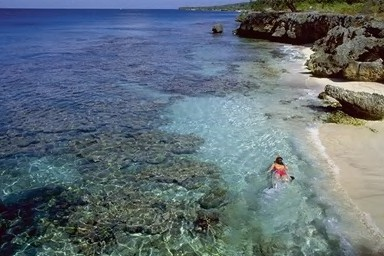
\includegraphics[width=\linewidth]{\detokenize{figuras/geracao/unsharp-a.png}}
  \caption{Original}
\end{subfigure}
\begin{subfigure}{.45\textwidth}
  \centering
  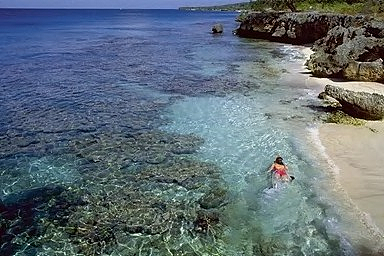
\includegraphics[width=\linewidth]{\detokenize{figuras/geracao/unsharp-b.png}}
  \caption{Imagem artificial}
\end{subfigure}
 \end{center}
 \caption[...]{\textit{Fonte:~Elaborado pela autora.}}
 \label{fig:gen:unsharp}
\end{figure}
Borra a imagem com um filtro Gaussiano, calcula a diferença entre a imagem original
e a imagem borrada e adiciona essa diferença na imagem original (Ver Algoritmo
\ref{alg:unsharp}). A imagem resultante (Figura \ref{fig:gen:unsharp}) é uma versão
realçada da imagem original, dado que soma à imagem justamente o que seria removido
com um filtro de suavização.

\vspace{0.5cm}
\begin{algorithm}[H]
  \caption{Algoritmo de aguçamento}
  \label{alg:unsharp}
  \SetAlgoLined
  \Entrada{Imagem colorida $I$ em formato BGR}
  \Saida{Imagem gerada $G$}
  \ParaCada{pixel $p$}{
    $\text{diferença} \gets I(p) - borrada(p)$\;
    $\text{G}(p) \gets I(p) + \text{diferença}$\;
  }
\end{algorithm}
\vspace{0.5cm}

\begin{description}
\item[Parâmetros e suas variações]
\item[Limitações]
\item[Métodos relacionados]
\item[Visualização]
\end{description}
%%%%%%%%%%%%%%%%%%%%%%%%%%%%%%%%%%%%%%%%%%%%%%%%%%%%%%%%%%%%%%%%%%%%%%%%%%%%%%%%
\section{Composição}

\vspace{0.5cm}
\begin{figure}
 \begin{center}
  \centering
  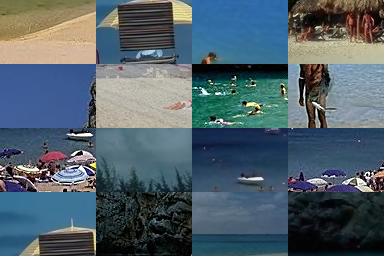
\includegraphics[width=0.5\linewidth]{\detokenize{figuras/geracao/composition.png}}
 \end{center}
 \caption[...]{\textit{Fonte:~Elaborado pela autora.}}
 \label{fig:gen:composition}
\end{figure}
\vspace{0.5cm}

Essa geração pretende considerar agrupar informações de várias imagens em uma única.
Acreditamos que o término brusco de uma imagem para início da outra ao formar a grade de imagens
tenha efeitos colaterais de inserção de textura que não excedam a vantagem de compor
uma mesma imagem com várias cores, texturas e formas das imagens originais.
\ref{fig:gen:composition}

\vspace{0.5cm}
\begin{algorithm}[H]
  \caption{Algoritmo de aguçamento}
  \label{alg:composition}
  \SetAlgoLined
  \Entrada{Imagem colorida $I$ em formato BGR}
  \Saida{Imagem gerada $G$}
\end{algorithm}
\vspace{0.5cm}

\begin{description}
\item[Parâmetros e suas variações]
\item[Limitações]
\item[Métodos relacionados]
\item[Visualização]
\end{description}
%%%%%%%%%%%%%%%%%%%%%%%%%%%%%%%%%%%%%%%%%%%%%%%%%%%%%%%%%%%%%%%%%%%%%%%%%%%%%%%%
\section{Mistura limiarizada}

\begin{figure}
 \begin{center}
\begin{subfigure}{.3\textwidth}
  \centering
  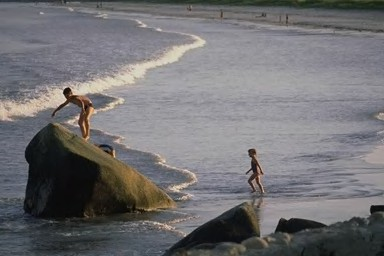
\includegraphics[width=\linewidth]{\detokenize{figuras/geracao/threshold-a.png}}
  \caption{Original}
\end{subfigure}
\begin{subfigure}{.3\textwidth}
  \centering
  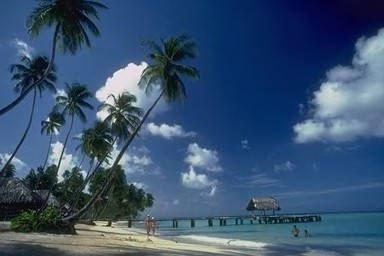
\includegraphics[width=\linewidth]{\detokenize{figuras/geracao/threshold-b.png}}
  \caption{Original}
\end{subfigure}
\begin{subfigure}{.3\textwidth}
  \centering
  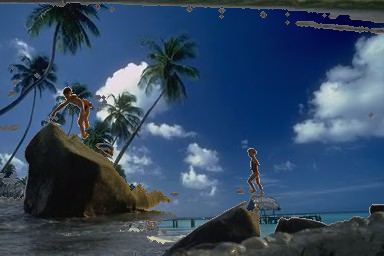
\includegraphics[width=\linewidth]{\detokenize{figuras/geracao/threshold-c.png}}
  \caption{Imagem artificial}
\end{subfigure}
 \end{center}
 \caption[...]{\textit{Fonte:~Elaborado pela autora.}}
 \label{fig:gen:threshold}
\end{figure}

A ideia da combinação de ``thresholds'' \ref{fig:gen:threshold} é compor uma nova
imagem que tenha como fundo (\textit{background}) uma imagem e como objeto de cena
(\textit{foreground}) de outra imagem.

\vspace{0.5cm}
\begin{algorithm}[H]
  \caption{Algoritmo de aguçamento}
  \label{alg:threshold}
  \SetAlgoLined
  \Entrada{Imagem colorida $I$ em formato BGR}
  \Saida{Imagem gerada $G$}
\end{algorithm}
\vspace{0.5cm}

\begin{description}
\item[Parâmetros e suas variações]
\item[Limitações]
\item[Métodos relacionados]
\item[Visualização]
\end{description}
%%%%%%%%%%%%%%%%%%%%%%%%%%%%%%%%%%%%%%%%%%%%%%%%%%%%%%%%%%%%%%%%%%%%%%%%%%%%%%%%
\section{Mistura saliente}

\begin{figure}
 \begin{center}
\begin{subfigure}{.3\textwidth}
  \centering
  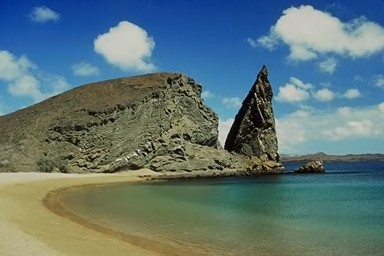
\includegraphics[width=\linewidth]{\detokenize{figuras/geracao/saliency-a.png}}
  \caption{Original}
\end{subfigure}
\begin{subfigure}{.3\textwidth}
  \centering
  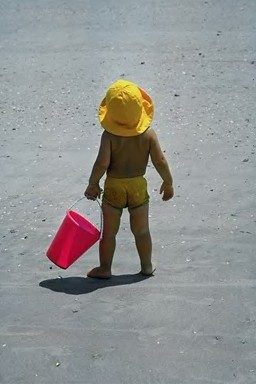
\includegraphics[width=\linewidth]{\detokenize{figuras/geracao/saliency-b.png}}
  \caption{Original}
\end{subfigure}
\begin{subfigure}{.3\textwidth}
  \centering
  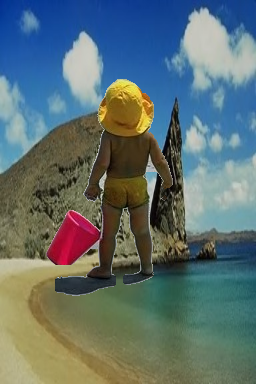
\includegraphics[width=\linewidth]{\detokenize{figuras/geracao/saliency-c.png}}
  \caption{Imagem artificial}
\end{subfigure}
 \end{center}
 \caption[...]{\textit{Fonte:~Elaborado pela autora.}}
 \label{fig:gen:saliency}
\end{figure}

Combinação de regiões salientes \ref{fig:gen:saliency}, muito similar com o método
anterior, porém, utilizando um algorítmo mais robuscado que detecta a saliência
da imagem.

\vspace{0.5cm}
\begin{algorithm}[H]
  \caption{Algoritmo de aguçamento}
  \label{alg:saliency}
  \SetAlgoLined
  \Entrada{Imagem colorida $I$ em formato BGR}
  \Saida{Imagem gerada $G$}
\end{algorithm}
\vspace{0.5cm}

\begin{description}
\item[Parâmetros e suas variações]
\item[Limitações]
\item[Métodos relacionados]
\item[Visualização]
\end{description}
%%%%%%%%%%%%%%%%%%%%%%%%%%%%%%%%%%%%%%%%%%%%%%%%%%%%%%%%%%%%%%%%%%%%%%%%%%%%%%%%
\section{SMOTE visual}

\begin{figure}
 \begin{center}
\begin{subfigure}{.3\textwidth}
  \centering
  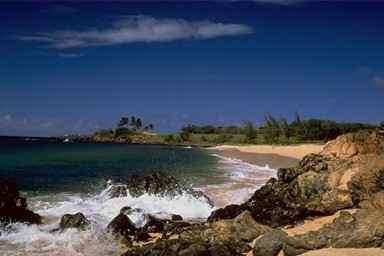
\includegraphics[width=\linewidth]{\detokenize{figuras/geracao/smote-a.png}}
  \caption{Original}
\end{subfigure}
\begin{subfigure}{.3\textwidth}
  \centering
  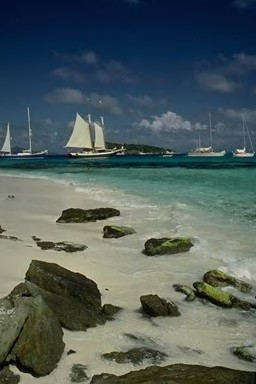
\includegraphics[width=\linewidth]{\detokenize{figuras/geracao/smote-b.png}}
  \caption{Original}
\end{subfigure}
\begin{subfigure}{.3\textwidth}
  \centering
  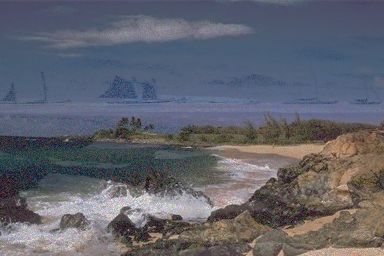
\includegraphics[width=\linewidth]{\detokenize{figuras/geracao/smote-c.png}}
  \caption{Imagem artificial}
\end{subfigure}
 \end{center}
 \caption[...]{\textit{Fonte:~Elaborado pela autora.}}
 \label{fig:gen:smotevisual}
\end{figure}

Conforme visto na seção x, o SMOTE é um método de rebalanceamento aplicado após
a extração de características. A ideia dessa geração, chamada de SMOTE visual,
é imitar esse funcionamento no nível de pixels. A diferença é que não é feito
entre as imagens mais próximas, mas sim entre duas imagens escolhidas de forma
aleatória do conjunto de treinamento da classe minoritária.
\ref{fig:gen:smotevisual}

\vspace{0.5cm}
\begin{algorithm}[H]
  \caption{Algoritmo da geração com SMOTE visual}
  \label{alg:smotevisual}
  \SetAlgoLined
  \Entrada{Imagem colorida $I$ em formato BGR}
  \Entrada{Imagem colorida $I_2$ em formato BGR}

  \Saida{Imagem gerada $G$}

  \ParaCada{pixel $p$}{
    $\text{diferença} \gets absoluto(I(p) - I_2(p))$\;
    $\text{gap} \gets \text{número aleatório entre 0 e 1}$\;
    $\text{G}(p) \gets I(p) + gap*\text{diferença}$\;
  }

\end{algorithm}
\vspace{0.5cm}

\begin{description}
\item[Limitações]
\item[Métodos relacionados]
\item[Visualização]
\end{description}
%%%%%%%%%%%%%%%%%%%%%%%%%%%%%%%%%%%%%%%%%%%%%%%%%%%%%%%%%%%%%%%%%%%%%%%%%%%%%%%%
\section{Adição de ruído}

\begin{figure}
 \begin{center}
\begin{subfigure}{.45\textwidth}
  \centering
  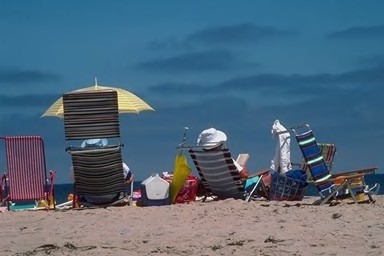
\includegraphics[width=\linewidth]{\detokenize{figuras/geracao/noise-a.png}}
  \caption{Original}
\end{subfigure}
\begin{subfigure}{.45\textwidth}
  \centering
  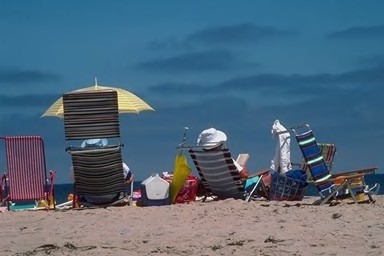
\includegraphics[width=\linewidth]{\detokenize{figuras/geracao/noise-a.png}}
  \caption{Imagem artificial}
\end{subfigure}
 \end{center}
 \caption[...]{\textit{Fonte:~Elaborado pela autora.}}
 \label{fig:gen:noise}
\end{figure}

O ruído de Poisson ocorre na contagem de fótons de dispositivos ópticos. Segue a distribuição
de Poisson que expressa a probabilidade de um certo número de eventos que ocorrem em um
intervalo fixo de tempo e/ou espaço se esses eventos ocorem com uma taxa média conhecida.
\ref{fig:gen:noise}
% \begin{equation}
% P_\mi)(n) = (e^(-\mi)\mi^(n))/(n!), n >= 0
% \end{equation}

\vspace{0.5cm}
\begin{algorithm}[H]
  \caption{Algoritmo da geração com ruído de Poisson}
  \label{alg:noise}
  \SetAlgoLined
  \Entrada{Imagem colorida $I$ em formato BGR}

  \Saida{Imagem gerada $G$}

  \ParaCada{pixel $p$}{
    $L \gets exp(-I(p))$\;
    $p \gets 1$\;
    $k \gets 0$\;
    {
    $k \gets k + 1$\;
    $p \gets p * \text{número aleatório entre 0 e 1}$\;

    } \Enqto {$p > L$}

    $\text{G}(p) \gets k - 1$\;
  }

\end{algorithm}
\vspace{0.5cm}

\begin{description}
\item[Parâmetros e suas variações]
\item[Limitações]
\item[Métodos relacionados]
\item[Visualização]
\end{description}
%%%%%%%%%%%%%%%%%%%%%%%%%%%%%%%%%%%%%%%%%%%%%%%%%%%%%%%%%%%%%%%%%%%%%%%%%%%%%%%%
% \section{Metodologia}
%
% \begin{description}
%  \item[Pesquisa bibliográfica:] \
%
%   \begin{enumerate}
% \item \underline{Características latentes}: são estudados diversos métodos de pré-processamento de imagens, como filtros de borramento e filtragem, com o objetivo de obter imagens processadas que sejam melhor caracterizadas para a etapa de classificação. O enfoque está em como realçar determinadas características, como, por exemplo, cor e textura, utilizando diversos algoritmos sobre as imagens originais.
%
% \item \underline{Redes neurais}: por representarem o estado da arte da classificação, reconhecimento e localização de objetos, as redes neurais de convolução são estudadas. Pretende-se utilizar a análise dos resultados do seu treinamento para identificar as características relevantes em imagens. Já as máquinas de Boltzmann restritas são redes neurais mais simples, portanto convenientes para a verificação da relevância de uma imagem para o aprendizado.
%
% \item \underline{Desbalanceamento de classes}: esse problema é fundamentado em reconhecimento de padrões, e consiste em lidar com um conjunto de classes que possuem quantidades desiguais de imagens. Deve-se assim pesquisar métodos que visam equilibrar o número de imagens em cada classe.
%
% \item \underline{Descritores}: são investigados métodos capazes de descrever as propriedades das imagens, como histograma global de cor (GCH)~\cite{Gonzalez2007}, vetor de coerência de cor (CCV)~\cite{ccv}, classificação de pixels de borda e interior (BIC)~\cite{bic}, auto-correlograma de cor (ACC)~\cite{acc} e descritores de Haralick~\cite{Haralick1973}.
%
% \item \underline{Classificador de padrões}: alguns classificadores fundamentados na literatura para a classificação de imagens são o Naive Bayes, OPF (\textit{Optimum-Path Forest}), KNN (\textit{K-Nearest Neighbor}), SVM (\textit{Support Vector Machines}) e Softmax. A depender da performance do sistema após experimentos um destes será escolhido. É importante destacar que esse não é o foco deste estudo, que tem a maior contribuição na pesquisa do pré-processamento das imagens de forma a obter características relevantes e no rebalanceamento de classes com dados de informação visual.
%   \end{enumerate}
%
%  \item[Implementação:] a biblioteca \-OpenCV \cite{Intel2010} será utilizada para as funções gerais de carregar, processar, salvar e classificar imagens. A linguagem de programação para utilizar esta biblioteca e na qual esta pesquisa está sendo implementada é C++. Para a geração de gráficos das medidas estatísticas a linguagem de programação Python é utilizada. O código está disponível em \url{https://bitbucket.org/moacirponti/imagefeatureextraction/overview}.
%
%  \item[Bases de imagens:] considerando que os objetivos propostos possuem um viés genérico, os experimentos vão ser realizados em diversas coleções de imagens com o objetivo de estabelecer ou refutar as hipóteses levantadas.
%
%  Os resultados preliminares foram obtidos utilizando a base de imagens COREL\footnote{Disponível em http://wang.ist.psu.edu/docs/related/}, composta por fotografias que representam as classes: tribos africanas, praia, construções, ônibus, dinossauros, elefantes, flores, cavalos, montanhas e tipos de comidas. São 10 classes balanceadas com 100 imagens cada. Para fins de exemplificação, foram selecionadas imagens que representam essas classes na Figura \ref{fig:corel}.
%
%  \begin{figure}[hbpt]
%  \begin{center}
%    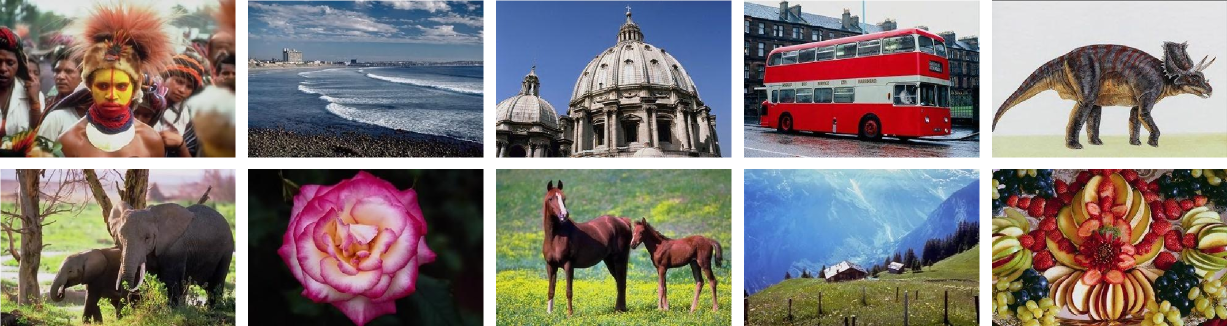
\includegraphics[width=1\linewidth]{\detokenize {figuras/exemplos_corel.png}}
%  \end{center}
%   \caption[Base de imagens COREL-1000.]{Base de imagens COREL-1000 utilizada. Estão representadas as 10 classes da base. \textit{Fonte: Elaborado pela autora.}}
%  \label{fig:corel}
% \end{figure}
%
%
%  \item[Experimentos:] serão realizados diversos experimentos direcionados a explorar as etapas de pré-processamento, para melhorar a acurácia da classificação de bases de imagens. Como entrada são utilizadas imagens originais provenientes de diversas coleções disponíveis na literatura. Como resultado, serão calculadas medidas estatísticas da classificação dessas coleções após a alteração dessas imagens com os métodos de realce de características relevantes.
%
%  \item[Análise dos dados:] os experimentos realizados irão resultar em medidas estatísticas da classificação. A análise irá comparar a classificação das imagens originais com aquelas tratadas pelo método proposto. Ainda, o método de rebalanceamento de classes será comparado com técnicas disponíveis na literatura, como o SMOTE.
%
% \item[Forma de avaliação:] a medida estatística mais comum para avaliação é a razão do número de acertos pela quantidade de imagens testadas. Essa medida, conhecida por \underline{acurácia}, pode não refletir propriamente os resultados, em um cenário de bases desbalanceadas. Isso se deve ao fato de que se a classe minoritária não obtiver nenhum resultado correto e a classe majoritária tiver 100\% de acertos, a acurária normal poderá ser muito alta, mesmo considerando que nenhuma imagem da classe minoritária foi corretamente classificada. Dessa forma, considera que os erros são igualmente importantes. Mas em se tratando de bases desbalanceadas, deve-se diferenciar o erro em, por exemplo, diagnosticar um paciente doente -- classe minoritária -- como sendo saudável e um paciente saudável -- classe majoritária -- como estando doente \cite{Batista2004}. No primeiro caso, o paciente corre risco de diagnóstico tardil, enquanto o paciente saudável realiza outros testes para refutação.
%
% Pode-se estender essa medida obtendo-se a \underline{acurácia $k$-fold}: medida de acerto baseada na divisão do conjunto de objetos em teste e treinamento, realizando a repetição dos experimentos $n$ vezes e obtendo a média e o desvio padrão. A acurácia de cada experimento é obtida pela Equação~\ref{eq:Accuracy}, que considera problemas de desbalanceamento de classes.
%
%     \begin{equation}
%       Acc = 1 - \frac{\sum_{i=1}^{c} E(i)}{2c},
%     \label{eq:Accuracy}
%     \end{equation}
%
%     \noindent onde $c$ é o número de classes e $E(i) = e_{i,1} + e_{i,2}$ é o erro relativo a $c$, calculado por:
%
%     \begin{equation*}
%       e_{i,1} = \frac{FP(i)}{N-N(i)} \,\,\,\,\, \text{ e } \,\,\,\,\, e_{i,2} = \frac{FN(i)}{N(i)}, i=1,...,c,
%     \label{eq:Errors}
%     \end{equation*}
%    \noindent onde $FN(i)$ (falsos negativos) são os exemplos pertencentes a $i$ e incorretamente classificados, e $FP(i)$ (falsos positivos) são os exemplos erroneamente rotulados como~$i$.
%
% % consideramos positivos a minoritaria
%
% Uma outra medida para bases desbalanceadas é a \underline{medida-F1} (conhecida como \textit{F1-Measure} ou \textit{F1-Score} e apresentada na Equação~\eqref{medidaf}), que combina precisão e revocação como medida de efetividade da classificação \cite{Garcia2009}.
% % Pode efetivamente avaliar a performance de classificação em cenários desbalanceados.
% A precisão (Equação~\ref{precisao}) é a medida da exatidão: dos exemplos classificados como positivos, quantos realmente são. E a revocação (Equação~\ref{revocacao}) é a medida de completude: quantos exemplos positivos foram corretamente classificados como tal.
%
% \begin{equation}
%   P = \frac{VP}{VP + FP},
%   \label{precisao}
% \end{equation}
%
% \noindent onde $VP$ são os exemplos positivos corretamente classificados.
%
% \begin{equation}
%   R = \frac{VP}{VP + FN}
%   \label{revocacao}
% \end{equation}
%
% \begin{equation}
%   F1 = 2 \frac{PR}{P+R}
%   \label{medidaf}
% \end{equation}
%
% A partir dessas medidas, o \underline{teste estatístico de Friedman} pode ser usado para determinar se há diferença significante em uma amostra de resultados gerados \cite{friedman2010}. As performances dos algoritmos são analisados e um \textit{rank} é atribuído para cada conjunto de dados. Ele considera que a hipótese nula a ser testada é que não há diferença estatística relevante entre as observações. Para analisar se o teste da hipótese é significativo, pode ser utilizado o \underline{p-valor}, que indica o quão estatisticamente significante o resultado é: quanto menor o seu valor, maior a evidência contra a hipótese nula (geralmente o limiar utilizado é de 0,05).
%
% Por fim, a \underline{distância de Mahalanobis} também pode ser utilizada: antes e depois da geração artificial de imagens, calcular a distância entre a média das classes e a variância dentro das classes \cite{mahalanobis2000}. Ela se baseia na correlação entre as variáveis e pode ser definida por
% \begin{equation*}
%   D_m(x_i) = \sqrt{(x_i - \mu)C^{-1}(x_i-\mu)^T},
% \end{equation*}
% \noindent onde $x_i$ é um vetor de valores, $\mu$ a média e C a matriz de covariância.
%
% \end{description}
%
% %--------------------------------------------------------------------------------
% \section{Resultados esperados}
% \label{sec:resultados}
%
% Os resultados esperados são relacionados às áreas de \textbf{processamento de imagens e reconhecimento de padrões}. Espera-se obter uma comprovação das hipóteses levantadas por essa pesquisa. Os resultados são esperados em duas vertentes:
%
% \begin{enumerate}
%  \item \textit{Pré-processamento} de imagens que caracterizem melhor aspectos de suas classes, aumentando a variância entre as classes quando comparado com as imagens originais.
%  \item \textit{Geração artificial de imagens} de classes minoritárias de forma a compensar o desbalanceamento natural das bases de dados.
% \end{enumerate}
%
% Em ambos os casos pretende-se melhorar a classificação, validando-a através do cálculo da medida-F1. A análise das características aprendidas por uma rede neural de convolução será realizada ao executar o treinamento com bases específicas que destaquem propriedades como cor, textura e forma. Além disso, os resultados serão obtidos a partir da escolha de quais imagens adicionam informação ao conjunto de treino. As redes RBM serão utilizadas para este fim. Bases naturalmente não balanceadas serão testadas e seus resultados avaliados.


%--------------------------------------------------------------------------------
\section{Considerações finais}

% A proposta desta pesquisa foi apresentada, descrevendo a sua metodologia. Foi dado destaque aos resultados esperados e à forma de avaliação, descrevendo as medidas estatísticas a serem utilizadas. O cronograma previsto para a realização deste mestrado foi destacado, elencando as atividades e suas respetivas durações. O próximo capítulo apresentará os resultados preliminares.
